\documentclass[../main.tex]{subfiles}

\begin{document}

\newcommand{\vertsep}{\unskip\ \vline\ } % = FIGURE | FIGURE - `\ ` and `\unskip` needed to align spacing

The U-Net was chosen to tackle this task. The U-Net is a convolutional neural network (CNN), first designed for medical image segmentation. The main characteristics of an U-Net are its ability to perform well with a relatively small amount of data and ability to train the upsampling process. The name comes from its shape - for each downsampling (convolution) operation, there is one upscaling operation, which when drawn out creates a 'U' shape.

For convoluting the image, a \emph{depthwise separable-convolution} (DSC) approach was chosen. This approach is characterized by splitting the spatial correlation and the cross-channel correlation into two convolutions.
The first convolution (depthwise) aims to reduce the dimensions of the input matrix, whilst preserving the channel count. The second convolution (pointwise) reduces the channel count using a $1\times 1$ kernel without changing the spatial properties of the matrix. This approach allows to train the spatial and cross-channel reasoning seperately.
At the end of each DSC, a ReLU layer is added to introduce non-linear behavior.

The model consists of 3 downsample-upsample blocks. The downsample part is made using some count of DSC-ReLU iterations on the input image, while only the first iteration changes the channel count, followed by a single MaxPool operation. Upsampling is done using some number of DSC-ReLU iterations with the last operation changing the channel count, followed by a single MaxUnpool operation.

The model was implemented in \code{Python 3.10} using \code{PyTorch} and \code{TorchLightning} libraries. The full source code of the model (along with the dataset) can be found on the GitHub repository.\footnote{\href{https://www.github.com/MBugdol/u-net-impl}{https://www.github.com/MBugdol/u-net-impl}}

The model summary can be seen in table \ref{tab:unet-summary}, and the model graph can be seen in figure \ref{fig:unet-graph}.

\begin{table}[htb]
	\centering

	\caption{U-Net summary (without batch dimension)}
	\label{tab:unet-summary}

	\newcommand{\dhline}{\hline\hline}

	\begin{tabularx}{1.0\textwidth}{
			| >{\hsize=0.8\hsize\linewidth=\hsize}X
			| >{\hsize=0.6\hsize\linewidth=\hsize}X
			| >{\hsize=1.3\hsize\linewidth=\hsize}X
			| >{\hsize=1.3\hsize\linewidth=\hsize}X
			|
		}
		\hline
		Type       & Params & Input sizes              & Output sizes             \\\dhline
		DownDSC    & 12.0 K & \texttt{[ 3 , 512, 512]} & \texttt{[64 , 256, 256]} \\\hline
		DownDSC    & 49.7 K & \texttt{[64 , 256, 256]} & \texttt{[128, 128, 128]} \\\hline
		DownDSC    & 253 K  & \texttt{[128, 128, 128]} & \texttt{[256, 64 , 64 ]} \\\hline
		UpDSC      & 256 K  & \texttt{[256, 64 , 64 ]} & \texttt{[128, 128, 128]} \\\hline
		UpDSC      & 51.2 K & \texttt{[128, 128, 128]} & \texttt{[64 , 256, 256]} \\\hline
		UpDSC      & 13.5 K & \texttt{[64 , 256, 256]} & \texttt{[ 4 , 512, 512]} \\\dhline
		Full U-Net & 637k   & \texttt{[ 3 , 512, 512]} & \texttt{[ 4 , 512, 512]} \\\hline
	\end{tabularx}
\end{table}

% Model graph page
\null
\vfill
\begin{figure}[htb]
	\centering
	\begin{subfigure}{0.45\textwidth}
		\centering
		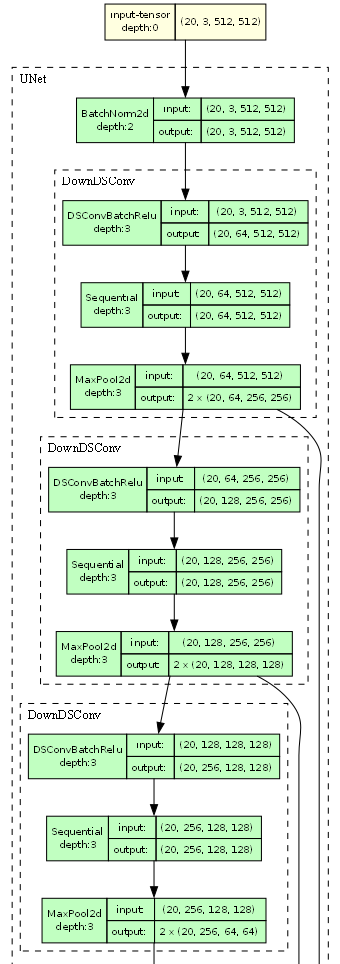
\includegraphics[height=.85\textheight]{model/model_graph_1.png}
	\end{subfigure}
	\vertsep
	\begin{subfigure}{0.45\textwidth}
		\centering
		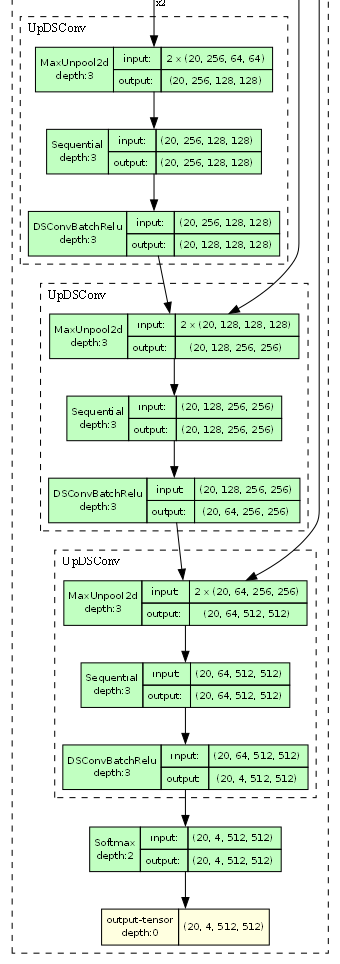
\includegraphics[height=.85\textheight]{model/model_graph_2.png}
	\end{subfigure}

	\caption{U-Net visualisation as a graph}
	\label{fig:unet-graph}
\end{figure}
\vfill
% End of model graph page


\end{document}